\documentclass[conference]{IEEEtran}
% Add the compsoc option for Computer Society conferences.
\usepackage{graphicx}
\usepackage{amsmath}
\usepackage[font=footnotesize,caption=false]{subfig}
\usepackage{algorithm}
\usepackage{algpseudocode}
\usepackage{booktabs}
% correct bad hyphenation here
\hyphenation{op-tical net-works semi-conduc-tor}


\begin{document}

\title{V4 Neural Network Model for Visual Saliency \\
and Discriminative Local Representation of Shapes}

\author{%\IEEEauthorblockN{Homer Simpson}\IEEEauthorblockA{Twentieth Century Fox}\and
\IEEEauthorblockN{Hui Wei and Zheng Dong}
\IEEEauthorblockA{Department of Computer Science, Laboratory of Cognitive Model and Algorithm, Fudan University\\
Shanghai Key Laboratory of Data Science, Fudan University\\
Shanghai, China\\
weihui@fudan.edu.cn}}

\maketitle

\begin{abstract}
Visual area V4 lies in the middle of the ventral visual pathway in the primate brain. 
It is an intermediate stage in the visual processing for object discrimination. 
It plays an important role in the neural mechanism of visual attention and shape recognition.
V4 neurons exhibit selectivity for salient features of contour conformation.
In this paper, we propose a novel model of V4 neurons based on a multilayer neural network
inspired by recent studies on V4.
Its low-level layers consist of computational units simulating simple cells and complex cells
in the primary visual cortex.
These layers extract preliminary visual features including edges and orientations.
The V4 computational units calculate the entropy of the extracted features 
as a measure of visual saliency.
The salient features are then selected and encoded with a layer of 
Restricted Boltzmann Machine to generate an intermediate representation of object shapes.
The model was evaluated in shape distinction, handwritten digits classification, feature detection, 
and feature matching experiments.
The results demonstrate that this model generates discriminative local representation
of object shapes.
It provides clues to understand the high level representation of visual stimuli in the brain.
\end{abstract}

\section{Introduction}

\PARstart{U}{nderstanding} the content of images has always been a difficult task 
in image analysis due to the well known semantic gap \cite{smeulders2000}
between low-level representation of images and the highly abstracted semantic 
content contained in the images.
However, biological brains accomplish this task accurately and effortlessly.
It is an attractive goal to understand the neural mechanism of vision in the brain
and simulate this mechanism with electronic computers.
Neuroscience studies in the past decades have provided us with the opportunity
to understand the neural processes of visual perception \cite{ungerleider2011}.

Visual stimuli captured by the eye are transformed into neural impulses in the retina 
and further processed by the visual cortex for high level cognitive tasks. 
The visual cortex plays an important role in filling the gap 
between visual stimuli and the implied semantic information.
Neural impulses travel through the visual pathways in the visual cortex 
and finally contribute to a unified percept of the object of interest.
Primate brains possess two distinct visual pathways \cite{ettlinger1990,lehky2007}.
The dorsal pathway is involved with processing the object's spatial location relevant to the viewer. 
The ventral pathway is involved with object discrimination and recognition.
In this paper, we concentrate on the latter, the ventral pathway, and visual area V4 in particular.

V4 lies in the middle of the ventral pathway (\figurename~\ref{fig:1}).
Lower levels of the pathway (visual areas V1 and V2) extract preliminary visual features 
including edges and orientations \cite{hubel1962,hubel1965}.
Higher levels of the pathway (inferior temporal cortex) exhibit selectivity to complex objects
like faces and body parts \cite{bruce1981,bell2009}.
As an intermediate stage, V4 plays a crucial role in transforming low-level orientation signals 
into complex object representations.

\begin{figure}[htp]
\centerline{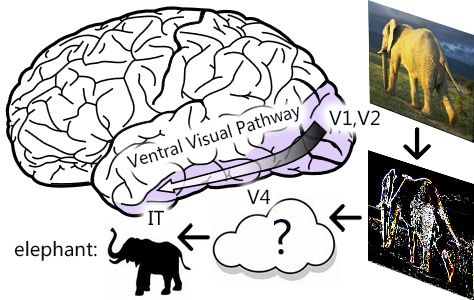
\includegraphics[width=0.8\linewidth]{images/fig1.png}} 
\caption{V4 is an intermediate stage in visual recognition.}
\label{fig:1}
\end{figure}

In the following section, we briefly introduce the neurobiological studies on V4 by which our model is inspired.
We also discuss several previous work on the computational models of V4 and their limitations.
In section \ref{sec:3}, we describe our model in details.
The proposed model is a multilayer neural network.
It extracts low-level orientation features from images and measures the visual saliency of the features.
The salient features are further encoded into discriminative local representation of object shapes.
In section \ref{sec:4}, the model is evaluated in a series of experiments.
The conclusion is summarized in section \ref{sec:5}.

\section{Related Work}
\label{sec:2}

\subsection{Shape Selectivity of V4 Neurons}

Neurobiological studies on V4 have not produced a unified model of its function or circuitry.
V4 neurons are known to be selective for color, shape, depth and even motion \cite{roe2012}.
In this paper, we focus on the V4 selectivity for shapes. 
Early experiments examined the selectivity of cells in V4 
with classical stimuli including bars and sinusoidal gratings~(\figurename~\ref{fig:2a}) \cite{desimone1987}.
Similar to earlier processing stages, some V4 neurons are tuned for orientation 
and spatial frequency of edges and linear sinusoidal gratings.
However, the majority of V4 neurons are sensitive to more complex shape properties. 
Later experiments demonstrated that V4 neurons display a clear bias in their responses 
in favor of non-Cartesian gratings~(\figurename~\ref{fig:2b}) and they show a significant degree of invariance 
in their selectivity across changes in stimulus position \cite{gallant1996}.
More recent experiments showed that V4 neurons can be strongly selective for curvature
of contours and angular position of acute curvatures \cite{pasupathy1999,pasupathy2001}. 
\figurename~\ref{fig:2c} shows a response map of a V4 neuron
(reproduced from \cite{pasupathy2001}).
The white shapes in \figurename~\ref{fig:2c} is presented in the receptive field of this V4 neuron
with equally dark background. 
The gray scale in the response map indicates the strength of the neuronal response.
Darker background indicates that the neuronal response is stronger.
This neuron is selectively tuned for acute convex border at the bottom left.
The curvature and the angular position are both necessary conditions of the activation of this neuron.
Neither rounded protrusions nor sharp curvatures towards directions other than the bottom left
activate the neuron.

\begin{figure}[htp]
\centering
\subfloat[]{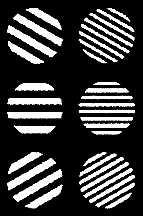
\includegraphics[width=0.18\linewidth]{images/fig2a.png}\label{fig:2a}}\hfil
\subfloat[]{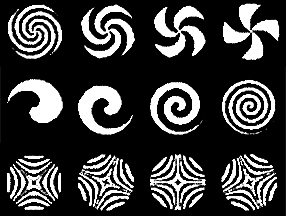
\includegraphics[width=0.36\linewidth]{images/fig2b.png}\label{fig:2b}}\hfil
\subfloat[]{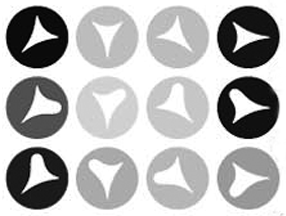
\includegraphics[width=0.36\linewidth]{images/fig2c.png}\label{fig:2c}}
\caption{Shapes to examine V4 selectivity.
(a) Classical gratings.
(b) Non-Cartesian gratings. V4 neurons prefer non-Cartesian gratings rather than classical gratings.
(c) Response map of a V4 neuron which responds to a sharp convex curvature at the bottom left.
Darker background indicates a stronger response.}
\label{fig:2}
\end{figure}

\subsection{Previous Models of V4}

Several models have been proposed to explain the shape selectivity and invariance of V4 neurons.
We briefly introduce the SRF model \cite{david2006} and the HMAX model \cite{riesenhuber1999,cadieu2007}.

The spectral receptive field (SRF) \cite{david2006}
describes properties of V4 receptive field in terms of the orientation and spatial frequency spectrum.
The model is based on the fact that V4 neurons have large orientation and spatial frequency bandwidth.
They respond selectively to stimuli such as contour conformations and non-Cartesian gratings,
which generally consist of multiple orientations and spatial frequencies.
The spectral model is also invariant to small changes in stimulus position 
and thus explains the invariance property of V4 response patterns.
The model is powerful in describing the shape selectivity of V4 neurons.
However, it does not explain the emergence of the selectivity.
It does not either provide the neural computing process to achieve such spectral receptive field.

The HMAX model was first proposed in \cite{riesenhuber1999}
as a generic model for object recognition in the visual cortex.
It models the visual cortex into a hierarchical architecture 
consisting of cascaded linear filters and non-linear maximum pooling operations.
It was then adopted as a model for V4 shape selectivity and invariance \cite{cadieu2007}.
The training of the model is an NP-complete problem. 
The authors used a greedy algorithm to obtain approximated solutions
but they did not provide any biological evidence for the algorithm. 

The proposed model of V4 in this paper overcomes the limitation of the previous models.
In the next section, we demonstrate that its architecture and function is analogous 
to those of the visual cortex.
We also provide efficient training method for our model.


\section{Neural Network Model of V4}
\label{sec:3}

The information processing in the visual cortex follows a hierarchical scheme.
Our model employs a similar hierarchical structure.
\figurename~\ref{fig:3} shows the architecture of our model.

\begin{figure}[htp]
\centerline{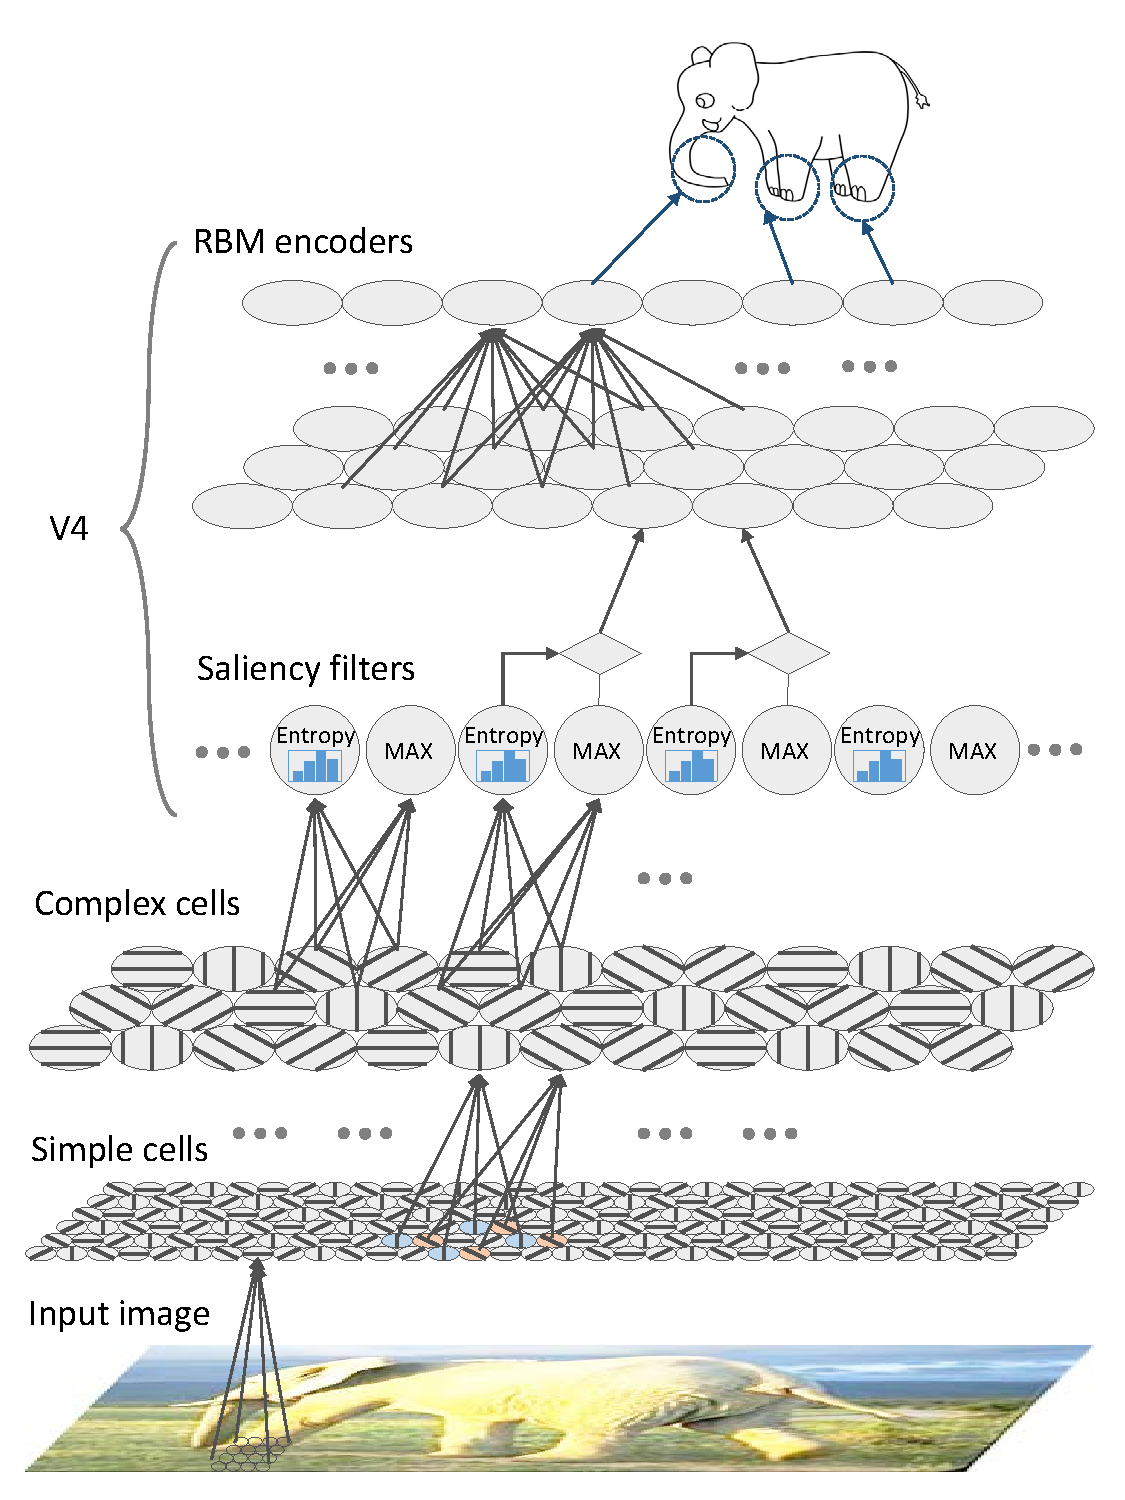
\includegraphics[width=0.99\linewidth]{images/fig3.pdf}} 
\caption{Multilayer neural network model of V4.}
\label{fig:3}
\end{figure}

In the feed-forward direction,
the first two layers consist of simple cells and complex cells
providing orientation features as input to V4 computation units.
The layer of saliency filters measures visual saliency in terms of the entropy of features.
Salient features are accurately located by maximizing neuronal response.
The extracted features are then further encoded into local representation of object shapes.

\subsection{Input Layers}

According to the hierarchy of the ventral visual pathway,
area V4 receives input from the lower levels including area V1 and V2.
These areas have been well studied since 1960s 
by Hubel, Wiesel \cite{hubel1962,hubel1965} and succeeding researchers.

Neurons in V1 and V2 respond to local orientations.
They fall into two categories, simple cells and complex cells.
Simple cells respond primarily to oriented edges and gratings.
Complex cells have larger receptive fields.
A stimulus is effective wherever it is placed in the complex receptive field, 
provided that the orientation is appropriate \cite{hubel1962}.

The receptive fields of simple cells can be understood as linear filters 
modeled as Gabor functions \cite{gabor1946},
\begin{equation}\label{equ:gabor}
g_{\theta,\sigma_s}(x,y)
=\exp \left(-\frac{x'^2+y'^2}{2\sigma_s^2}\right)
\cos \left(2\pi\frac{x'}{\lambda}\right),
\end{equation}
where $x'=x\cos\theta+y\sin\theta$, $y'=-x\sin\theta+y\cos\theta$.
In the equation, $\theta$ represents the preferred orientation,
$\sigma_s$ approximates the radius of the receptive fields,
and $\lambda$ is the wavelength of the sinusoidal factor.
$\lambda$ controls the spatial frequency of the filter.
In this paper, it is taken according to the scale of the filter
($\lambda=1.3\sigma_s$).

\begin{figure}[htp]
\centering
\subfloat[Odd symmetry]{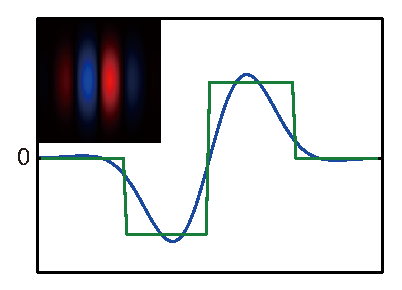
\includegraphics[width=0.45\linewidth]{images/fig4a.eps}\label{fig:4a}}\hfil
\subfloat[Even symmetry]{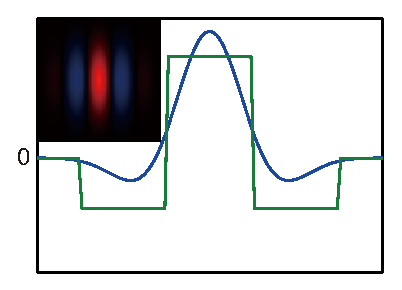
\includegraphics[width=0.45\linewidth]{images/fig4b.eps}\label{fig:4b}}
\caption{Different Gabor functions.}
\label{fig:4}
\end{figure}

In our model, the layer of simple cells operates on raw image input
(\figurename~\ref{fig:3}). 
The output of simple cells with preferred orientation $\theta$
and scale $\sigma_s$ is the following convolution
passed through a transfer function $\phi$,
\begin{equation}\label{equ:gabor}
S_{\theta,\sigma_s}(x,y)=\phi(I\otimes g_{\theta,\sigma_s}),
\end{equation}
where $I$ is an image and 
\begin{equation}\label{equ:gabor}
\phi(u)=\left\{\begin{array}{ll}
u & \text{if } u>0,\\
0 & \text{otherwise.}
\end{array}\right.
\end{equation}
A complex cell sums up the output of the simple cells in its receptive field, 
weighted with a Gaussian function,
\begin{equation}
f_{\sigma_c}(x,y)=\frac{1}{2\pi\sigma_c}\exp\left(-\frac{x^2+y^2}{2\sigma_c^2}\right),
\end{equation}
where $\sigma_c$ is the scale of complex cells.
Complex receptive field is usually 2 to 5 times larger than simple receptive field \cite{movshon1978}
and therefore in this paper, we have $\sigma_c=2\sigma_s$.

In section \ref{sec:4},
we show experimentally that complex cells provide sufficient information 
for the V4 model to form the selectivity for shapes.

\subsection{Saliency Filters}

V4 is an area of attentional modulation \cite{roe2012}.
Visual attention involves selecting an interested region or selecting specific object features.
Visual attention in V4 is influenced by both top-down feedback from higher levels in the visual pathway
and bottom-up input from lower levels.
We focus on the bottom-up influence.
In a bottom-up process, V4 evaluates the saliency of the input from lower levels
and focuses its attention automatically on the salient features.

We use entropy to measure the saliency of images \cite{kadir2001}.
In \cite{kadir2001}, it is assumed that salient regions have high complexity (and correspondingly high entropy).The entropy of features is used as a scale invariant measure.
The salient region is selected at entropy peaks over scales.
To avoid erroneously selecting noise or texture as salient regions,
a measure of self-similarity is employed.
Self-similar regions are filtered out.

In this paper, we use entropy in a different approach.
V4 neurons encode fragments of object contour \cite{pasupathy2001,pasupathy2002}.
They are selective for simple structures such as convex or concave curvature.
Therefore, in our assumption, 
well ordered structures with low complexity are preferred in cognitive activities.
We filter out regions with high complexity (or entropy).

The entropy is calculated according to the output of complex cells.
Given a point $(x,y)$, in the neighborhood of $(x,y)$,
a complex cell with preferred orientation $\theta$ has output value $C_{\theta}(x,y)$,
We suppose that the probability of a complex cell being activated
is proportional to the output value.
The probability is thus defined as:
\begin{equation}
P(\theta)=\frac{1}{\sum_{\theta_i} C_{\theta_i}(x,y)}\cdot C_{\theta}(x,y).
\end{equation}
The entropy of the complex cell activity in this neighborhood
is 
\begin{equation}
E=-\sum_{\theta} P(\theta) \log P(\theta).
\end{equation}

\figurename~\ref{fig:5} shows four image patches.
For each image patch, the output values of complex cells with different preferred orientations
(from $0^\circ$ to $180^\circ$) are plotted in a bar chart.
The charts show the distribution of complex cell activities.
The entropy calculated accordingly indicates that 
patches composed of simple structures have non-uniform distributions and thus low entropy values.
Therefore, we filter out regions with high entropy.

\begin{figure}[htp]
\centerline{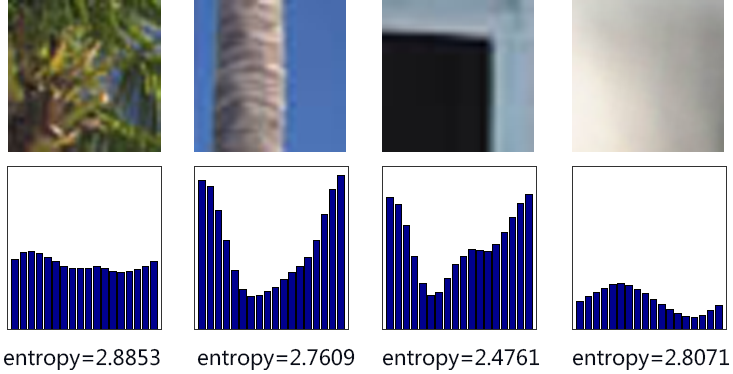
\includegraphics[width=0.8\linewidth]{images/fig5.png}} 
\caption{Entropy of image patches.
Bar charts in the second row show the output values of complex cells
with different preferred orientations (from $0^\circ$ to $180^\circ$).}
\label{fig:5}
\end{figure}

In addition to entropy, 
local competition also plays a role in attentional selection \cite{desimone1995}.
With limited neural resources, only strong and competitive neuronal signals get transmitted and processed.
In our model, the saliency layer finds local maximums of complex cell output
and filters out those points with high entropy values or low activities (or output values).
The algorithm is listed in Algorithm \ref{alg:1}.

\begin{algorithm}[htp]
  \caption{Saliency filter}
  \label{alg:1}
  \begin{algorithmic}[1]
    \Procedure{FindSalientPoint}{image $I$, scale $\sigma_c$, threshold $t_A,t_E$}
      \For{each orientation $\theta$}
        \State $C_{\theta}\leftarrow\phi(I\otimes g_{\theta})\otimes f_{\sigma_c}$
        \Comment{complex cell output}
      \EndFor
      \For{each point $(x,y)$ in image $I$}
        \State $C(x,y)\leftarrow\max_{\theta}C_{\theta}(x,y)$
        \State $E(x,y)\leftarrow$ entropy at point $(x,y)$
      \EndFor
      \State Divide image $I$ into patches of size $\sigma_c\times\sigma_c$
      \For{each patch $p$}
        \State $(\hat{x},\hat{y})\leftarrow\operatorname{argmax}_{(x,y)\in p}C(x,y)$
        \If{$C(\hat{x},\hat{y})>t_A$ and $E(\hat{x},\hat{y})<t_E$}
          \State Mark $(\hat{x},\hat{y})$ as a salient point
        \EndIf
      \EndFor
    \EndProcedure
  \end{algorithmic}
\end{algorithm}

\subsection{RBM Encoders}

With saliency filters described in the previous subsection,
we are able to focus on a limited number of salient points.
The V4 computation units in our model encode the shape in the neighborhood of each salient point.
The encoding is achieved with Restricted Boltzmann Machine (RBM).

RBM can learn a probability distribution over its set of inputs.
It has been found efficient in training deep neural network \cite{hinton2006}.
The encoder layer in our model is part of a deep network.
Therefore, we use the RBM as a training model for this encoder layer.
The RBM is trained to encode shape features in the neighborhood of a salient point.
\figurename~\ref{fig:6} shows such an RBM encoder.

\begin{figure}[htp]
\centerline{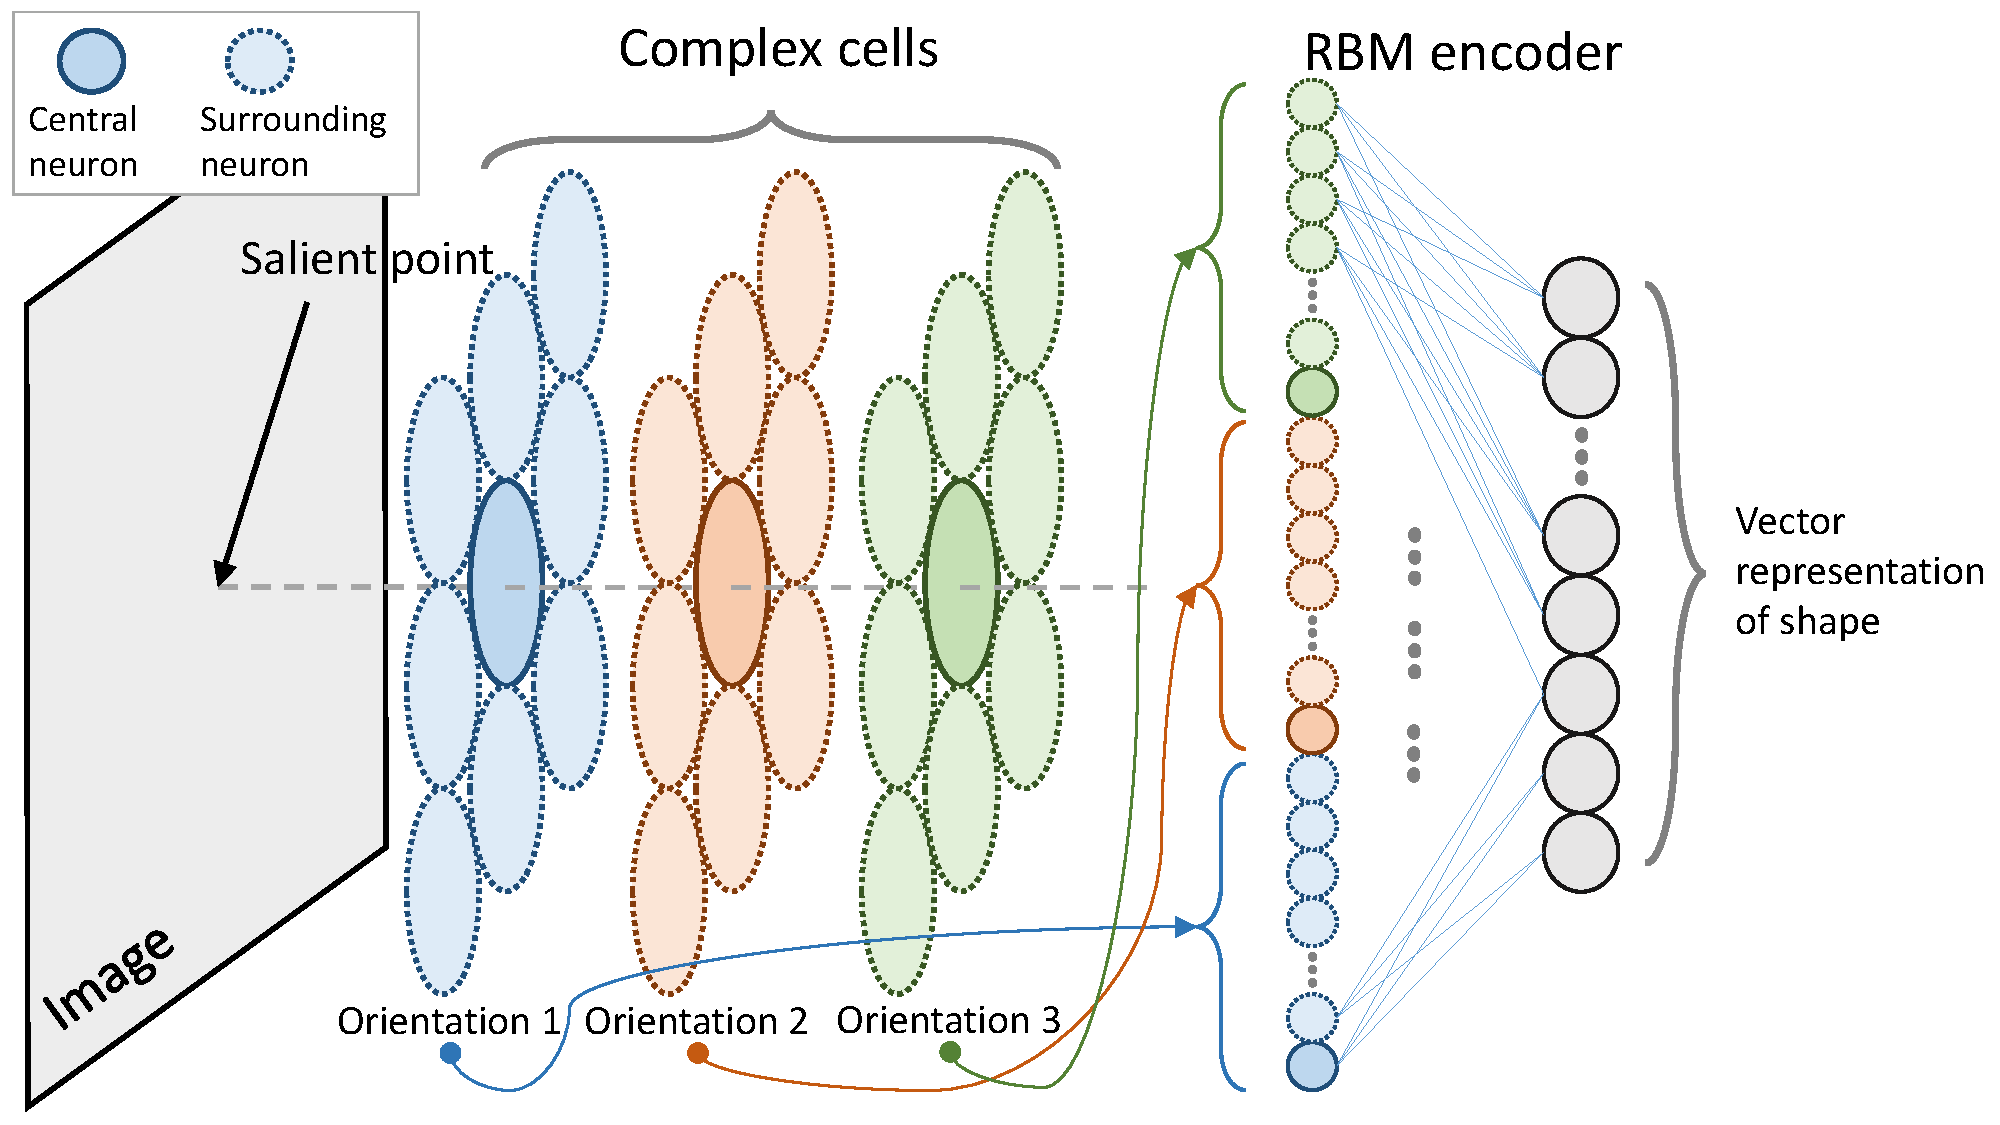
\includegraphics[width=0.99\linewidth]{images/fig6.pdf}} 
\caption{RBM encoder for local shape feature.}
\label{fig:6}
\end{figure}

Let $(x,y)$ denote a salient point.
For each preferred orientation, 
we select the complex cell of which the receptive field is centered at point $(x,y)$,
and its eight neighbors.
\figurename~\ref{fig:6} demonstrates an example of three preferred orientations.
In this case, $9\times3$ complex cells are selected.
The number of selected neurons depends on the number of orientations we choose.
The selected complex cells are then used as the input layer (or visible layer) of the RBM.
The representation of the shape in the neighborhood of $(x,y)$
is formed in the output layer (or hidden layer) of the RBM.

RBM can be trained efficiently with a contrastive divergence learning algorithm \cite{hinton2002}.
Let $w_{ij}$ be the weight of the connection from the $i$-th visible unit to the $j$-th hidden unit.
In each learning iteration, the change in the weight is given by
\begin{equation}
\Delta w_{ij}=\epsilon\left(\langle v_i h_j\rangle_\text{data}-\langle v_i h_j\rangle_\text{recon}\right),
\end{equation}
where $\epsilon$ is a learning rate, 
$\langle v_i h_j\rangle_\text{data}$ is the product of two units when the visible layer is given real data,
and $\langle v_i h_j\rangle_\text{recon}$ is the product of two units 
when the visible layer is given reconstructed data.

We use weight-decay \cite{hinton2010}
to reduce overfitting by adding an L2 penalty term, $\frac{1}{2}\lambda w^2$.
The weight change is then given by
\begin{equation}
\Delta w_{ij}=\epsilon\left(\langle v_i h_j\rangle_\text{data}-\langle v_i h_j\rangle_\text{recon}\right)
-\epsilon\lambda w_{ij},
\end{equation}
where $\lambda$ is a weight-cost coefficient.
We followed \cite{hinton2010} for the choice of the coefficient $\lambda$ and the learning rate $\epsilon$
in our experiments.

The output vector of the hidden layer forms a representation of local shape features.
It can be used directly as input for classification tasks.
We can also use the RBM connection weight matrix to initialize a multilayer neural network
for supervised back-propagation training.

\subsection{Model Parameters}

The size of the receptive field increases along the hierarchy of the visual system.
Lower levels have relatively small receptive fields while higher levels have larger receptive fields.
The size of receptive field in our model follows the same scheme.
The relationship is shown in Table \ref{tab:1}.
V4 neurons receive afferent connections from $3\times3$ complex cells
that have partially overlapped receptive fields.
Therefore the radius of the V4 receptive field is not 3 times as long as that of the complex cell.

\begin{table}[h]
\caption{Size of receptive field}
\centering
\begin{tabular}{rr}
\toprule
Category & Radius of receptive field \\
\midrule
Simple cells & $\sigma_s$ \\
Complex cells & $\sigma_c = 2\sigma_s$ \\
V4 RBM encoders & $2.5\sigma_c$\\
\bottomrule
\end{tabular}
\label{tab:1}
\end{table}

We used two schemes for the number of different preferred orientations of simple cells and complex cells.
For black and white images of shapes and handwritten digits in our experiment,
we used 4 orientations (from $0^\circ$ to $135^\circ$ in steps of $45^\circ$).
For gray scale images, we used 18 orientations (from $0^\circ$ to $170^\circ$ in steps of $10^\circ$)
in order to preserve more information.

The output of complex cells was normalized to the $[0,1]$ interval
to serve as the input of RMB encoders.
The saliency filters took a threshold $t_E=2.8$ for the entropy
and a threshold $t_A=0.4$ for complex cell output value (or complex cell activity).
These values were roughly the median values of natural images.

\section{Experiments}
\label{sec:4}

In this section, we demonstrate a series of experiments in which we evaluated our model.

\subsection{Perceptron over Complex Cells}

We have reviewed the shape selectivity of V4 neurons in section \ref{sec:2}.
In the following experiment, 
We examined that the output of complex cells provides sufficient information
for the emergence of neuronal response pattern of V4.
A single perceptron was trained to distinguish between two shapes (\figurename~\ref{fig:7a}).
The shapes were also used to examine the selectivity of V4 in \cite{pasupathy2001}.
The difference between the two shapes is that one has a sharp projection towards the top right.

\begin{figure}[htp]
\centering
\subfloat[Response map]{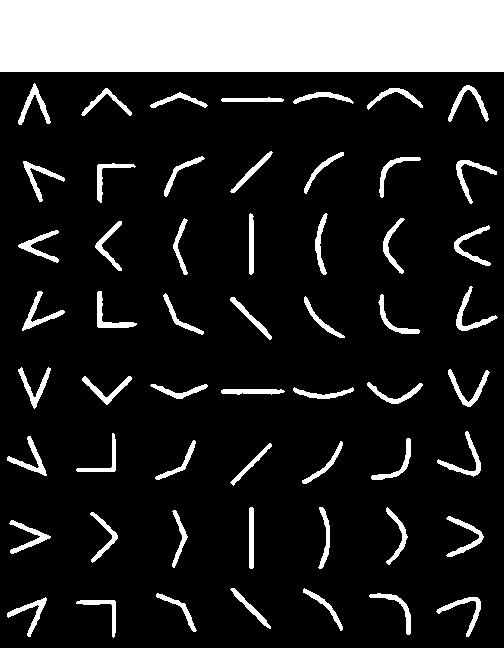
\includegraphics[width=0.48\linewidth]{images/fig7a.png}\label{fig:7a}}\hfil
\subfloat[Weight matrices]{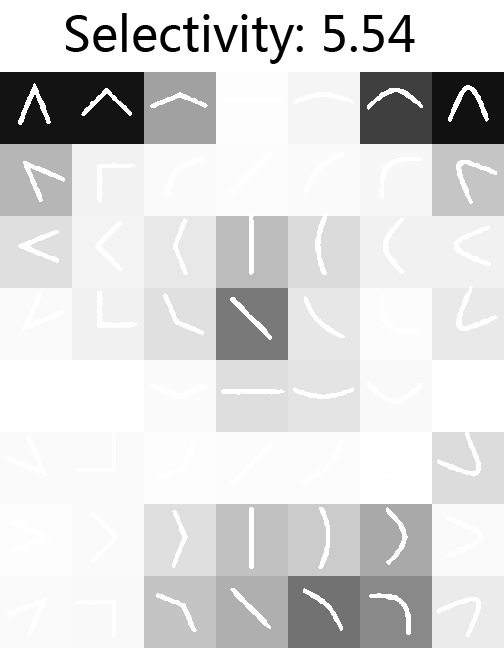
\includegraphics[width=0.48\linewidth]{images/fig7b.png}\label{fig:7b}}
\caption{Response map and weight matrices of a perceptron that distinguishes two shapes.
(a) Responses of the perceptron over 18 samples.
The perceptron prefers the shape in the left half of the samples.
It is insensitive to stimulus position.
(b) The input weight of the perceptron. 
Each block shows the weight of connections from complex cells of a certain orientation.
Complex cells of 18 different orientations provide input for this perceptron.}
\label{fig:7}
\end{figure}

Since V4 neurons show a certain degree of invariance in their selectivity across changes in stimulus position,
we moved the shapes randomly within the receptive field of the perceptron 
to generate samples for training and testing (\figurename~\ref{fig:7a} shows several samples).
The samples were then used as input of the layers of simple cells and complex cells.
The output of complex cells were passed to the perceptron.
We had complex cells with different preferred orientations 
(from $0^\circ$ to $170^\circ$ in steps of $10^\circ$) and over different positions in the receptive field.
Therefore, the input of the perceptron consisted of 18 matrices, 
each corresponding to the output of complex cells with a certain orientation.
The input weight of the perceptron was thus also 18 matrices.

The trained perceptron exhibited a strong bias towards the shape with convex curvature towards the top right.
It also showed a significant degree of invariance to the stimulus position.
It is obvious that the selectivity is not formed from certain excitatory sub-regions
or inhibitory sub-regions of the receptive field which was found of simple cells \cite{hubel1962,pasupathy2001}.
The selectivity of the perceptron tallies with the selectivity of actual V4 neurons.
The response map is shown in \figurename~\ref{fig:7a}.
Darker background colors indicate stronger responses.
The input weight of this perceptron is shown in \figurename~\ref{fig:7b}.
Each block shows the weight from the complex cells of a certain preferred orientation.
Red color denotes positive weight while blue color denotes negative weight.

This experiment demonstrates that complex cells provide sufficient information
for V4 neurons to show selectivity observed in neurobiological experiments.

\subsection{Shape Selectivity}

In the following experiment, we trained our model to learn shapes.
The training samples were collected from \cite{gallant1996,pasupathy1999,pasupathy2001}, 
including 4 categories of stimuli, i.e.,
sinusoidal gratings, non-Cartesian gratings, segmented curves, and closed shapes.
The simple cells in our model took these sample images as input.
The images were processed by simple cells and complex cells.
Since the sample images were fitted into V4 receptive fields in neurobiological experiments,
we adjusted the scale of the images to fit the size of a single V4 receptive field in our model too.
Therefore the saliency filters were not necessary in this experiment.
The output of complex cells were passed directly on to an RBM encoder.

We used an RBM with 256 hidden units (RBM output neurons) in this experiment.
In order to assess the selectivity of these units,
we assigned each unit a selectivity index over a category of stimuli.
The selectivity index is defined as the ratio of the maximal response to the average response 
over the stimuli of a certain category.
Given an RBM output unit $h$ and its output value $h_i$ over a category of $N$ stimuli for $i=1,2,\dots,N$.
The selectivity index $\mathcal{S}$ of $h$ is given by
\begin{equation}
\mathcal{S}(h)=\frac{\max\{h_i|i=1,2,\dots,N\}}{\sum_{i=1}^N h_i/N}.
\end{equation}
In the following statistics, we assumed that a neuron has significant selectivity over a category of stimuli
if the selectivity index is greater than 3.5.
Among the 256 units, 171 units exhibited significant selectivity for different stimuli.
102 units showed selectivity for segmented curves (\figurename~\ref{fig:8}).
55 units showed strong bias towards non-Cartesian gratings (\figurename~\ref{fig:9})
while 50 units showed selectivity for classical sinusoidal gratings.
68 units exhibited selectivity for closed shapes (\figurename~\ref{fig:10}).
The shape selectivity of our model is listed in \tablename~\ref{tab:2}.
The categories of selectivity are not mutually disjoint.
A single unit may possess more than one kind of selectivity simultaneously.

\begin{table}[h]
\caption{Shape selectivity of our model}
\centering
\begin{tabular}{rrr}
\toprule
Selectivity & Number of Units & Percentage \\
\midrule
Sinusoidal gratings & 50 & 19.5\% \\
Non-Cartesian gratings & 55 & 21.5\% \\
Segmented curves & 102 & 39.8\% \\
Closed shapes & 68 & 26.6\% \\
\bottomrule
\end{tabular}
\label{tab:2}
\end{table}

\begin{figure}[htp]
\centering
\subfloat[Patterns]{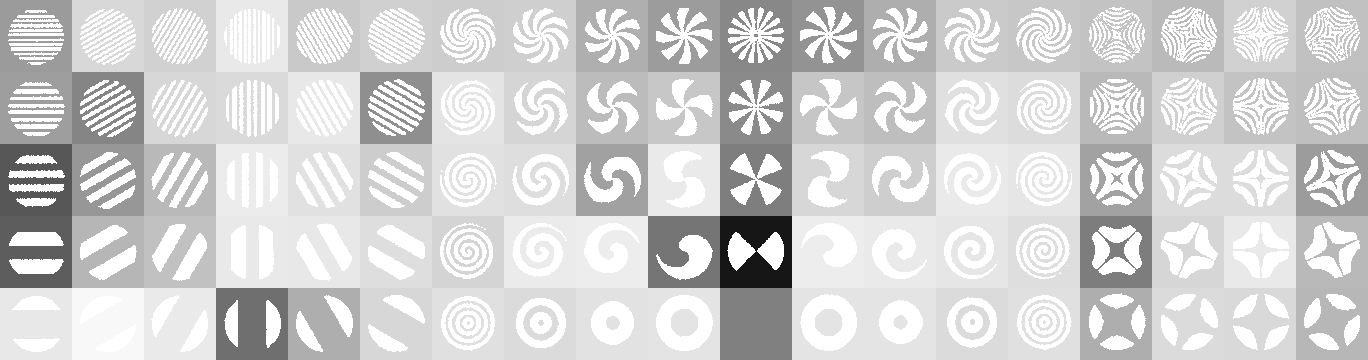
\includegraphics[width=0.24\linewidth]{images/fig8a.png}\label{fig:8a}}\hfil
\subfloat[Response map]{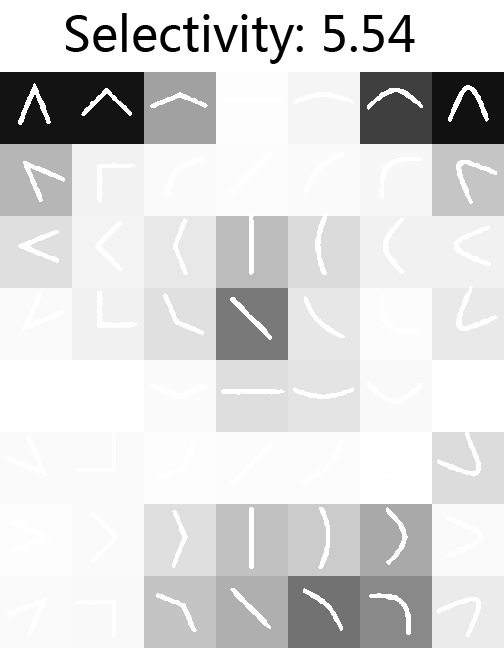
\includegraphics[width=0.24\linewidth]{images/fig8b.png}\label{fig:8b}}\hfil
\subfloat[Response map]{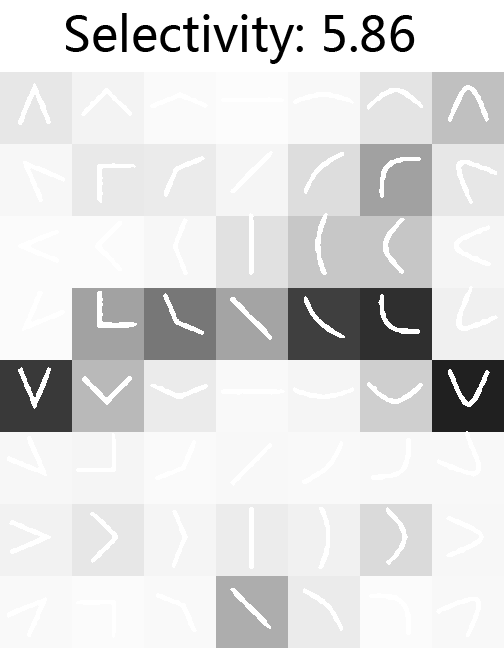
\includegraphics[width=0.24\linewidth]{images/fig8c.png}\label{fig:8c}}\hfil
\subfloat[Response map]{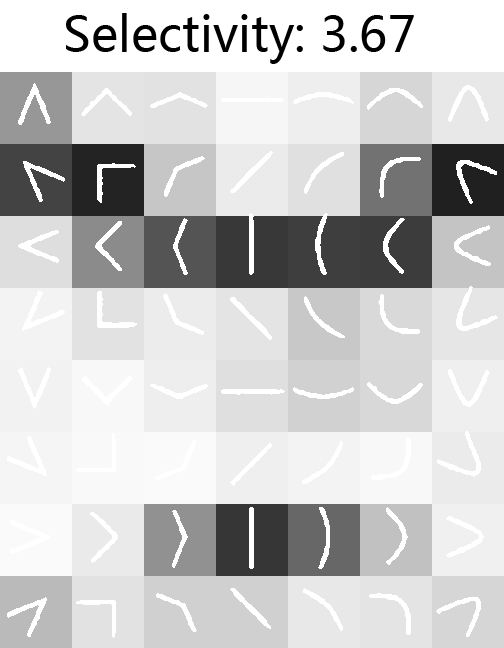
\includegraphics[width=0.24\linewidth]{images/fig8d.png}\label{fig:8d}}
\caption{RBM output neurons responding to convex curves towards certain directions.
(a) Sample patterns of segmented curves.
(b) Response map of a neuron tuned for curves projecting upwards.
(c) Response map of a neuron tuned for curves projecting downwards.
(d) Response map of a neuron tuned for curves projecting towards the top left.}
\label{fig:8}
\end{figure}

\figurename~\ref{fig:8a} shows the sample patterns of segmented curves.
\figurename~\ref{fig:8b} to \figurename~\ref{fig:8d} show the response maps of 3 RBM output neurons.
Darker background indicates stronger response.
The selectivity indexes is shown at the top.
It is shown that the three neurons exhibited strong bias towards curves rather than straight lines.
The neurons were tuned for the orientation of the projection of the segmented curves.
This is compliant with the selectivity of V4 neurons described in \cite{pasupathy1999}.

\begin{figure}[htp]
\centering
\subfloat[Response map of a neuron selective for a pair of circular sectors (selectivity index = 3.92).]%
{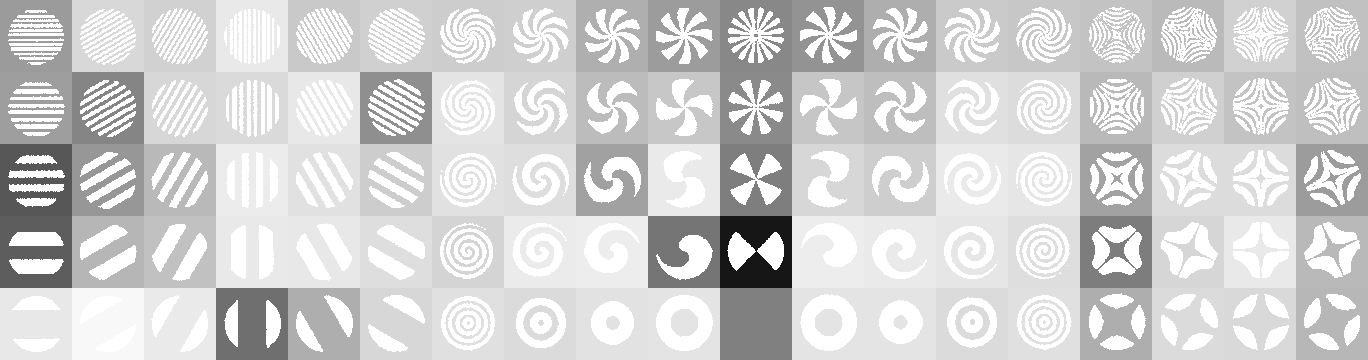
\includegraphics[width=0.9\linewidth]{images/fig9a.png}\label{fig:9a}}\\
\subfloat[Response map of a neuron selective for helix shapes (Selectivity index = 6.37).]%
{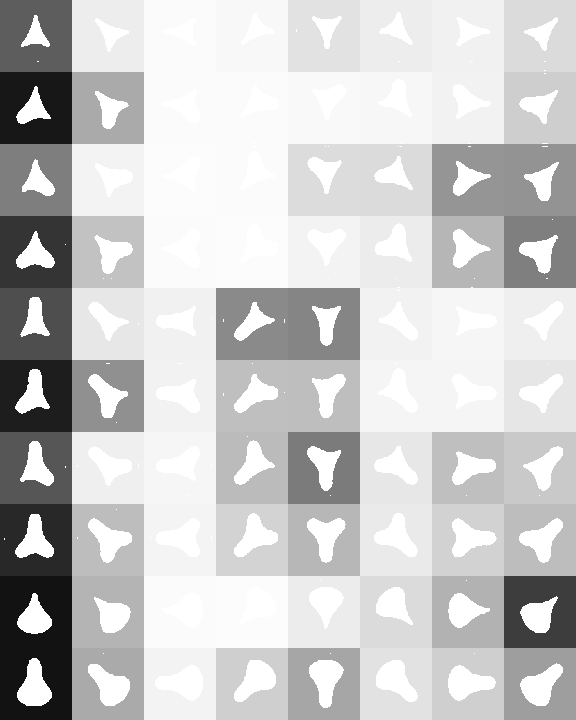
\includegraphics[width=0.9\linewidth]{images/fig9b.png}\label{fig:9b}}
\caption{Response maps of RBM output neurons tuned for non-Cartesian gratings.}
\label{fig:9}
\end{figure}

\figurename~\ref{fig:9} shows the response maps of two RBM output neurons
which are selective for non-Cartesian gratings.
Both of the two neurons were not sensitive to sinusoidal gratings.
The one in \figurename~\ref{fig:9a} was selective for a pair of circular sectors.
The one in \figurename~\ref{fig:9b} preferred non-Cartesian gratings of helix shapes.

\figurename~\ref{fig:10} shows the sample patterns of closed shapes and the response map of two neurons.
The two neurons were selectively tuned for two kinds of shapes.
They were sensitive to the angular position of the shapes.

\begin{figure}[htp]
\centering
\subfloat[Patterns]{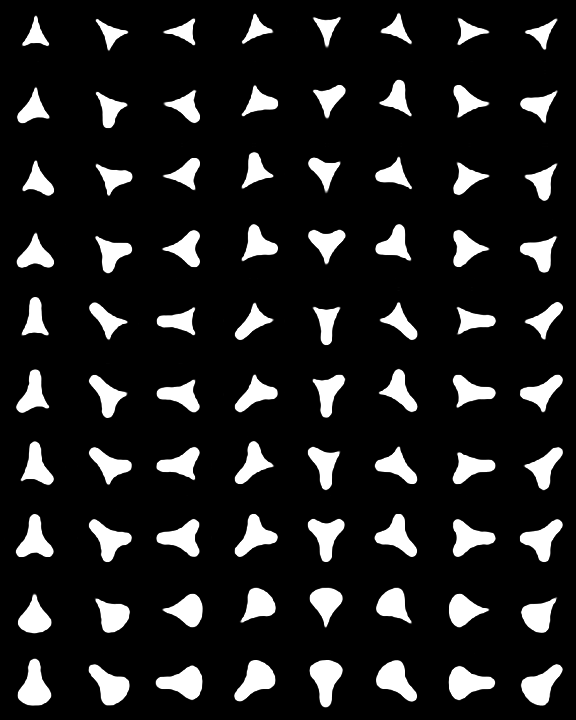
\includegraphics[width=0.31\linewidth]{images/fig10a.png}\label{fig:10a}}\hfil
\subfloat[Response map]{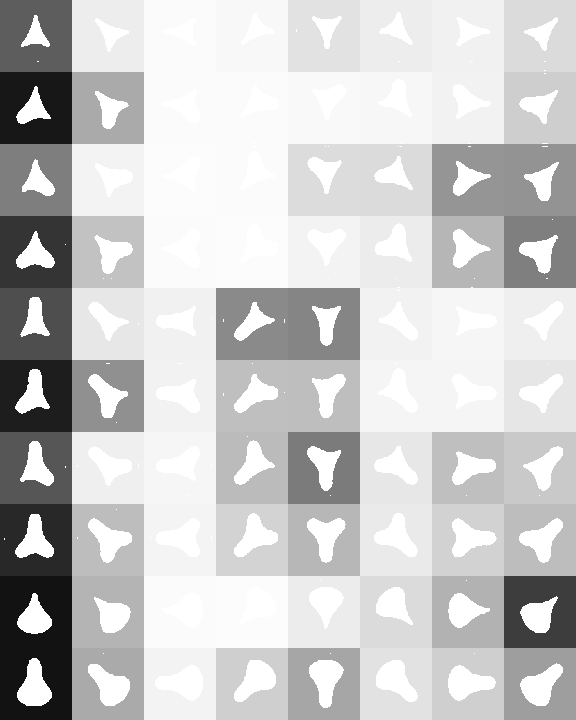
\includegraphics[width=0.31\linewidth]{images/fig10b.png}\label{fig:10b}}\hfil
\subfloat[Response map]{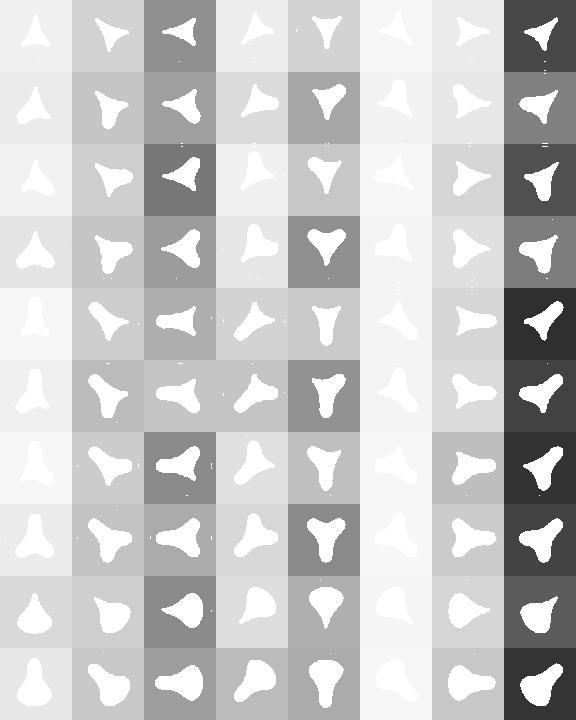
\includegraphics[width=0.31\linewidth]{images/fig10c.png}\label{fig:10c}}
\caption{RBM output neurons responding to closed shapes.}
\label{fig:10}
\end{figure}

This experiment demonstrates that our model can learn to distinguish the stimuli
which V4 neurons are selectively tuned for.

\subsection{Classifying Handwritten Digits}

In the following experiment,
we evaluated our model on the MINST database of handwritten digits \cite{lecun1998}.
We added another layer of artificial neurons over the RBM output
to classify handwritten digits.

The images of digits are $28\times28$ pixels in size.
We fitted the images into a single V4 receptive field thus the saliency filters were also bypassed in this experiment.

Since the images are black and white, we used complex cells with 4 preferred orientations, 
from $0^\circ$ to $135^\circ$ in steps of $45^\circ$.
Thus the input layer of the RBM encoder consisted of $4\times9$ units.
The output layer consisted of 128 units.
We added another layer of 10 units to be the binary classifiers of the digits (from 0 to 9).
These layers formed a $36\times128\times10$ feed-forward network.
We trained the RBM encoder with the training set of data.
The weight matrix of the RBM encoder was then used to initialize 
the weight between the first two layers of the network.
The network was then fine-tuned with back-propagation (BP) algorithm \cite{rumelhart2002}.
We also trained the network directly with back-propagation algorithm for a comparison.
\figurename~\ref{fig:11} shows the training error.
When the network was initialized with the RBM encoder of our model,
the BP training began with a significantly smaller training error.

\begin{figure}[htp]
\centering
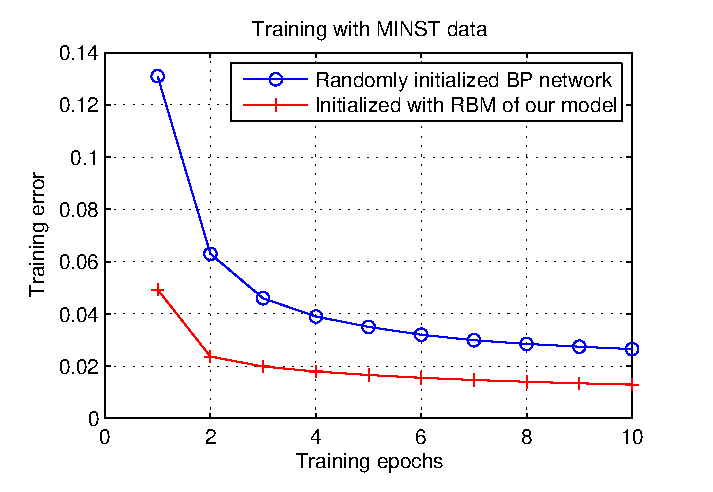
\includegraphics[width=0.7\linewidth]{images/fig11.eps}
\caption{Training error is smaller when using the RBM encoder to initialize the BP network.}
\label{fig:11}
\end{figure}

The test error of our model is also competitive compared with other algorithms.
A comparison is shown in Table \ref{tab:3}.
The benchmark is provided in \cite{lecun1998}.

\begin{table}[h]
\caption{Comparison of performance on MINST database}
\centering
\begin{tabular}{rr}
\toprule
Methods & Test error rate (\%) \\
\midrule
Our model & 2.9 \\
K-nearest neighbors & 5.0 \\
40 PCA + quadratic classifier & 3.3 \\
2-layer neural network & 4.7 \\
SVM, Gaussian kernel & 1.4 \\
\bottomrule
\end{tabular}
\label{tab:3}
\end{table}

\subsection{Feature Detection}

In the above experiments, the images contain very limited information.
They are small enough to fit into the receptive field of V4 computation unit.
When we deal with larger images, especially natural images,
we have to find some regions of interest 
and focus the computation units over a limited number of interesting regions.
A full scan over the whole image is not computationally economic.
It also complicates succeeding processing for high-level tasks 
such as object recognition and scene understanding.
The visual neural system takes a similar approach.
As we have reviewed in previous sections, 
V4 is closely related with selective visual attention \cite{roe2012}.
Research shows that V4 receptive field shrinks and shifts towards saccade target \cite{hamker2006}.
We simulated such visual attention with the saliency filters in our model.
In the following experiment,
we evaluated the saliency filters with feature detection experiment.

\begin{figure}[htp]
\centering
\subfloat[Car image]{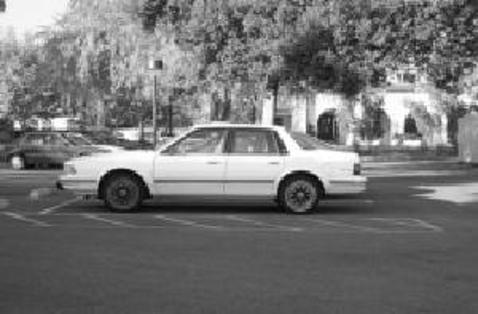
\includegraphics[width=0.32\linewidth]{images/fig12a.png}\label{fig:12a}}\hfil
\subfloat[Activity map]{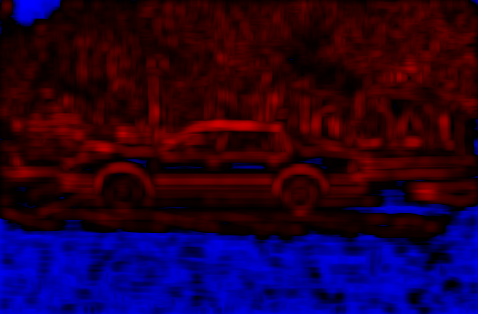
\includegraphics[width=0.32\linewidth]{images/fig12c.png}\label{fig:12b}}\hfil
\subfloat[Entropy map]{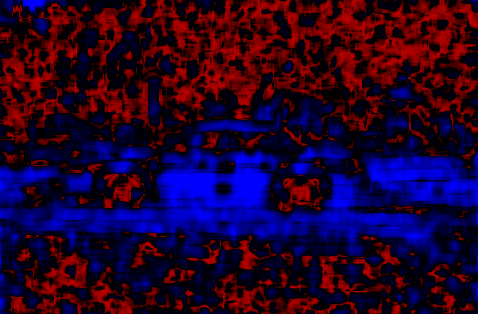
\includegraphics[width=0.32\linewidth]{images/fig12e.png}\label{fig:12c}}\\
\subfloat[Face image]{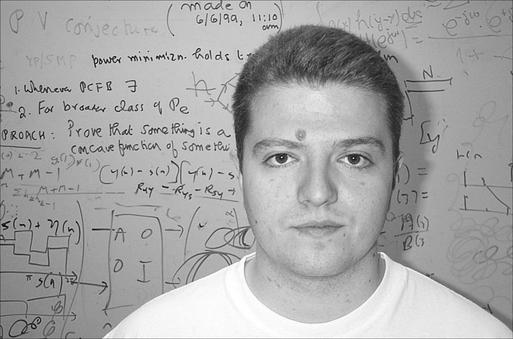
\includegraphics[width=0.32\linewidth]{images/fig12b.png}\label{fig:12d}}\hfil
\subfloat[Activity map]{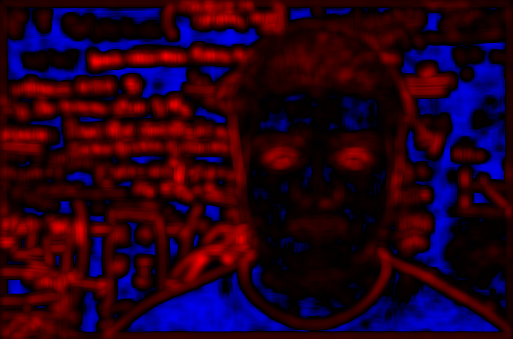
\includegraphics[width=0.32\linewidth]{images/fig12d.png}\label{fig:12e}}\hfil
\subfloat[Entropy map]{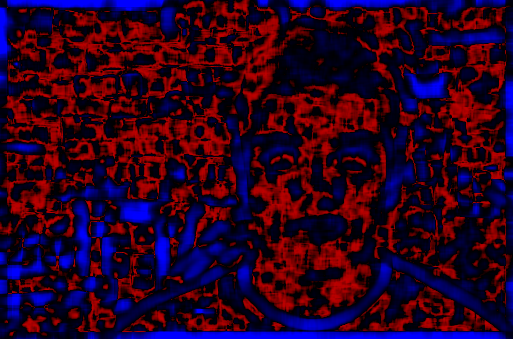
\includegraphics[width=0.32\linewidth]{images/fig12f.png}\label{fig:12f}}\\
\subfloat[Salient points]{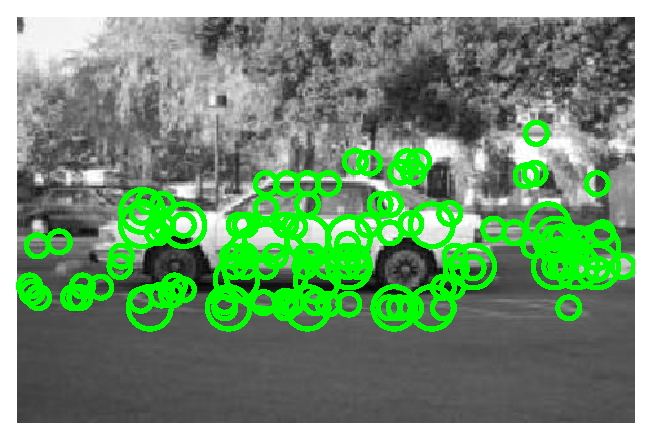
\includegraphics[width=0.49\linewidth]{images/fig12g.eps}\label{fig:12g}}\hfil
\subfloat[Salient points]{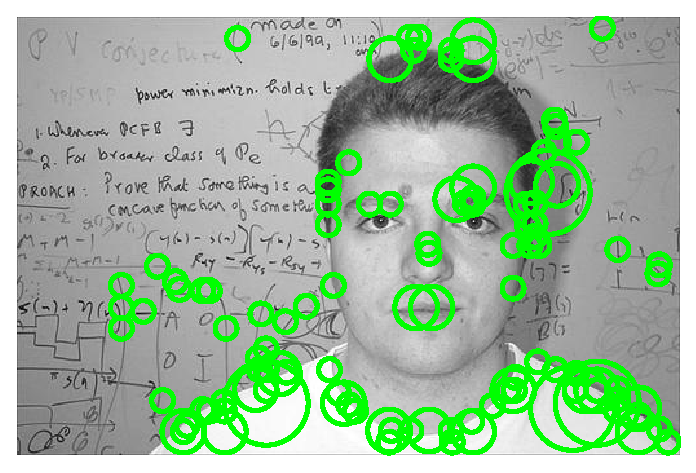
\includegraphics[width=0.49\linewidth]{images/fig12h.eps}\label{fig:12h}}
\caption{Feature detection. (a) and (d) show the original images.
(b) and (e) are the complex cell activity. 
Red color indicates strong activity and blue color indicates inhibition.
(c) and (f) are the entropy map.
Red color indicates high entropy value and blue color indicates low entropy value.
(g) and (h) are the selected salient points
at the scale of 4, 8, and 16 in terms of simple cell radius.}
\label{fig:12}
\end{figure}

\figurename~\ref{fig:12} shows the process of feature detection with the saliency filters in our model.
\figurename~\ref{fig:12b} and \figurename~\ref{fig:12d} show the activity map of complex cells.
The activities are high in the region of the trees behind the car (\figurename~\ref{fig:12a})
and the handwriting on the white board (\figurename~\ref{fig:12c}).
Saliency filters filter out these regions because these regions have a comparatively high entropy.
These areas consist of a large amount of disordered edges
which result in a near uniform distribution of complex cell activity over preferred orientations
and thus high entropy values.
The saliency filters can find salient points at each given scale.
\figurename~\ref{fig:12g} and \figurename~\ref{fig:12h} show the salient points
at the scale of 4, 8, and 16 in terms of the simple cell radius
(The size of the other units can be inferred with the relationship
shown in Table \ref{tab:1}).

\subsection{Feature Matching}

Previous work on feature matching emphasizes on matching 
physical points on the same object under different views (e.g. \cite{brown2011}).
The human vision has better generalization ability at feature matching
in that we can match the same part of different objects of some certain category
despite the minor differences in details.
This ability is important for learning the semantic of objects.
The following feature matching experiment demonstrates
that our model exhibits this kind of generalization ability.

In this experiment, we trained our model 
with images randomly selected from the Caltech data set \cite{fei2007}.
We took the output of the RBM encoders as the feature descriptors of the salient points.
A match between points from two images was then established by finding pairs of features
with minimal Euclidean distance.
The matches with feature distances greater than a threshold value (1.25 in this experiment)
were filtered out as non-matches.
The feature matching result between face images is demonstrated in \figurename~\ref{fig:13}.
Correct matches were established between different images of the same face.
Different faces were also matched because they were visually similar.

\begin{figure}[htp]
\centering
\subfloat[The same face]{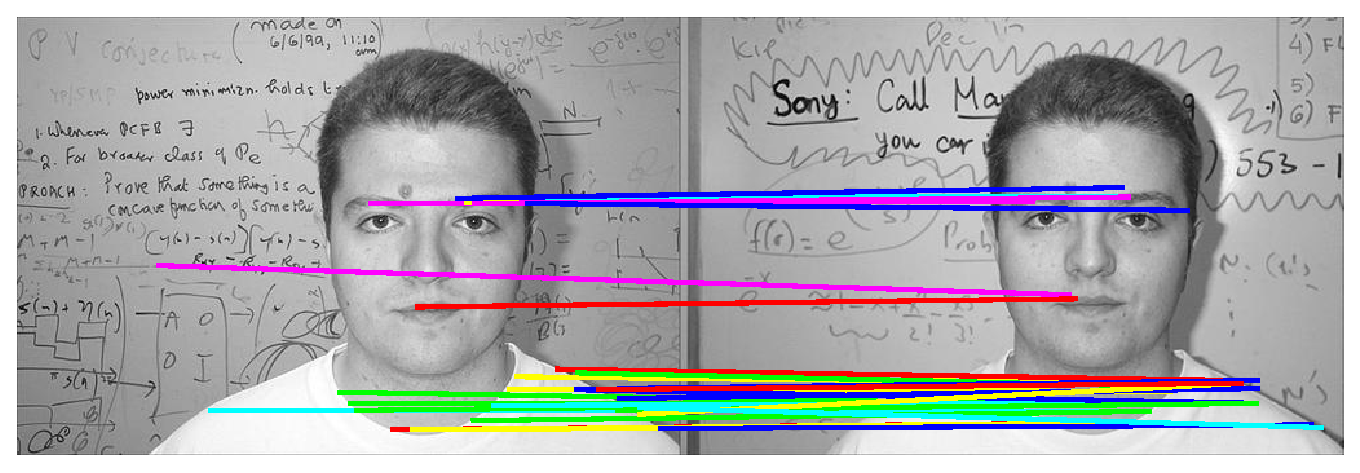
\includegraphics[width=0.85\linewidth]{images/fig13a.eps}\label{fig:13a}}\\
\subfloat[Different faces]{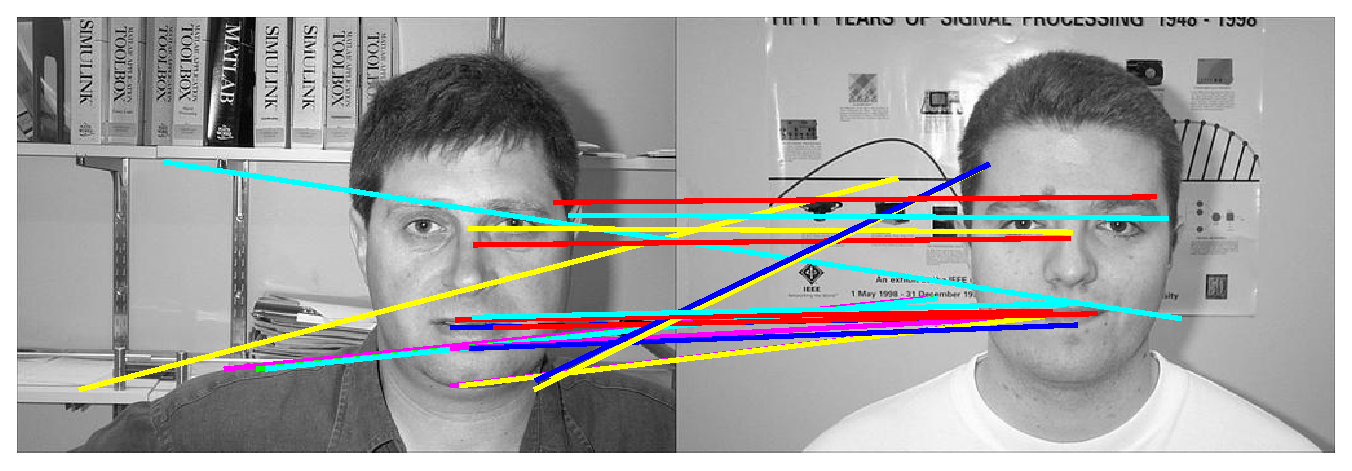
\includegraphics[width=0.85\linewidth]{images/fig13b.eps}\label{fig:13b}}
\caption{Feature matching result between face images.}
\label{fig:13}
\end{figure}

The comparison in \figurename~\ref{fig:14} demonstrates the advantage of our model.
We used SIFT feature \cite{lowe2004} for comparison.
\figurename~\ref{fig:14a} shows that our model produced correct matches between 
the model van in the left and the two real vans in the right.
However, SIFT feature failed to produce correct matches (\figurename~\ref{fig:14b}).
SIFT feature utilizes the direction of image gradient.
It fails to capture the shape feature of an object when the object's color changes dramatically
because the direction of image gradient changes with the color.
Our model focuses on the shape feature and thus achieves a stable matching despite the change in color.

\begin{figure}[htp]
\centering
\subfloat[Our matches]{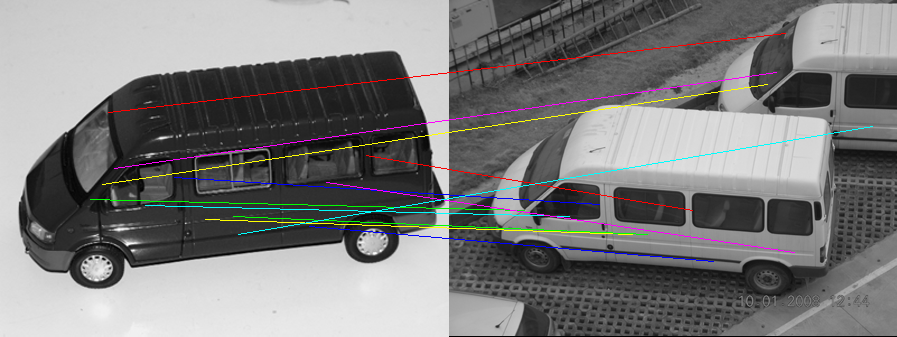
\includegraphics[width=0.99\linewidth]{images/fig14a.png}\label{fig:14a}}\\
\subfloat[SIFT matches]{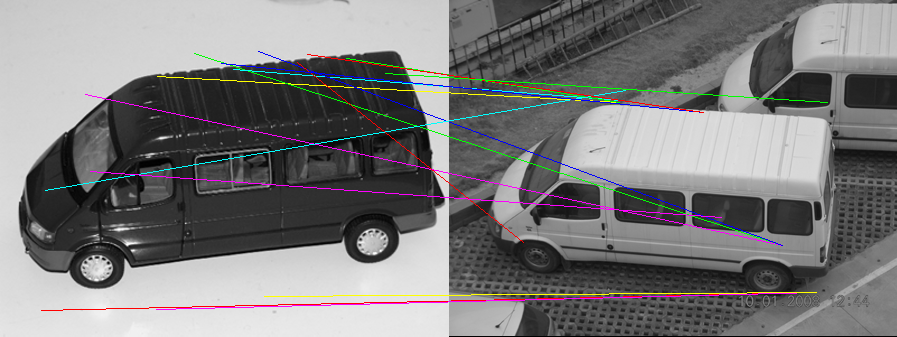
\includegraphics[width=0.99\linewidth]{images/fig14b.png}\label{fig:14b}}
\caption{Comparison of feature matching between van images.}
\label{fig:14}
\end{figure}

\section{Conclusion}
\label{sec:5}

In this paper, we propose a model for the visual area V4.
It is based on the neural mechanism of the ventral visual pathway.
We focus on visual attention and shape selectivity in V4.
V4 in our model is implemented as a multilayer neural network 
which selects salient points and encodes the shape feature in the neighborhood of the salient points.
We demonstrate a variety of experiments in which the model was evaluated.
The results show that the proposed model is consistent with the shape selectivity of area V4.
It can find salient points in images and encode local shape feature into a discriminative representation.

Future work should involve further quantitative evaluations of our model.
We will also investigate the application of our model in computer vision tasks
such as object recognition and scene understanding.

\section*{Acknowledgment}

This work was supported by the 973 Program (Project No. 2010CB327900), 
the NSFC project (Project No. 61375122, 81373556), 
and the National ``Twelfth Five-Year Plan'' for Science and Technology (Project No. 2012BAI37B06).

\bibliographystyle{IEEEtran}
\bibliography{IEEEabrv,ref}

\end{document}


